\chapter{Konzept von JUUT}

In diesem Kapitel wird ein möglicher Erstentwurf für das Test-Framework vorgestellt, der als Grundlage für die konkrete Implementierung dienen soll.

Zunächst betrachte ich aber die Struktur des schon existierenden Frameworks UUnit und möchte dessen Implementierung analysieren.

\section{Struktur von UUnit}

In diesem Abschnitt werde ich die Struktur von UUnit - stellvertretend für die existierenden Test-Frameworks für Unity - vorstellend und die Implementierung grob analysieren. Die daraus gewonnenen Erkenntnisse möchte ich für meinen Erstentwurf nutzen.

Auf der nächsten Seite befindet sich ein Klassendiagramm aller Klassen von UUnit und dessen relevanten Methoden. Wie man sieht besteht das Framework aus nur wenigen Klassen, wobei der Großteil der Arbeit von \textit{UUnitTestSuite} und \textit{UUnitTestCase} verrichtet wird.

\textit{UUnitTestCase} ist die Basisklasse aller Testklassen und stellt die Methoden \textit{SetUp} und \textit{TearDown} zur Verfügung, welche vor/nach jedem Aufruf eines Tests ausgeführt werden. \textit{testMethodName} repräsentiert den Namen der Testmethode, welche durch die Methode \textit{Run} gestartet werden soll. Bei der Ausführung eines Tests (s. \autoref{code:UUnitTestCase_Run} \nameref{code:UUnitTestCase_Run}) wird zunächst die \textit{SetUp}-Methode ausgeführt. Anschließend wird die auszuführende Testmethode per Reflection aufgerufen. Falls währenddessen eine Exception auftritt wird diese aufgefangen und deren Nachricht über die Debug-Konsole von Unity ausgegeben. Abschließend wird \textit{TearDown} ausgeführt. Im Zuge dessen wird auch das übergebene \textit{UUnitTestResult}-Objekt aktualisiert, wobei lediglich die Anzahl der ausgeführten und fehlgeschlagenen Tests angepasst werden.

\clearpage
\begin{figure}
\centering
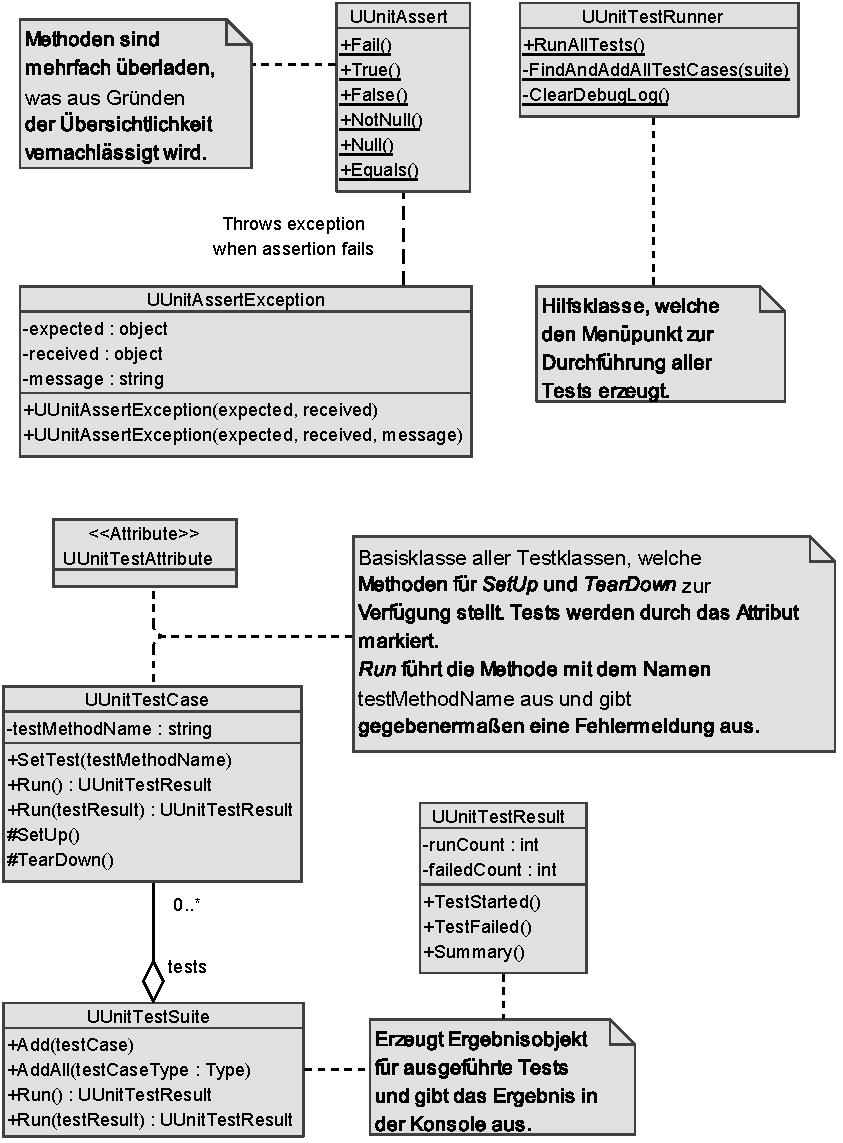
\includegraphics[width=0.9\linewidth]{images/Kapitel_ErstentwurfDesFrameworks/UUnitStruktur}
\caption[Struktur des Test-Frameworks UUnit]{Struktur des Test-Frameworks UUnit}
\label{fig:UUnitStruktur}
\end{figure}
\clearpage

\textit{UUnitTestSuite} verwaltet eine Menge von Testklassen, die per \textit{Add} und \textit{AddAll} hinzugefügt werden können. Aus dem Quellcode (s. \autoref{code:UUnitTestSuite_AddAll} \nameref{code:UUnitTestSuite_AddAll}) der \textit{AddAll}-Methode geht hervor, dass für jede einzelne Testmethode eine Instanz von \textit{UUnitTestCase} benötigt wird. Wird nun die \textit{Run}-Methode aufgerufen, wird zunächst eine \textit{UUnitTestResult} Instanz erzeugt. Anschließend wird von jedem enthaltenen \textit{UUnitTestCase} die \textit{Run}-Methode aufgerufen, wobei das Ergebnis-Objekt übergeben. Dieses wird abschließend an den Aufrufer zurückgegeben.

Ich halte es für unnötig, dass für jede einzelne Testmethode eine Instanz der Testklasse benötigt wird, sondern denke dass eine Instanz pro Testklasse logischer wäre. Außerdem ist ein leichtes Hinzufügen weiterer Tests nur über die \textit{AddAll}-Methode möglich, da die Methode zum Hinzufügen einer einzelnen Testmethode einen Parameter vom Typ \textit{UUnitTestCase} erwartet. Dadurch muss der Anwender eine Instanz seiner konkreten Testklasse erzeugen und das Attribut \textit{testMethodName} korrekt fülle, um einen einzelnen Test hinzuzufügen. Diesen Umstand halte ich für nicht intuitiv. Des Weiteren denke ich, dass die Ausführung aller für Tests relevanten Methoden in einer separaten Klasse besser aufgehoben wäre und nicht in \textit{UUnitTestCase} gehört. Auch die direkte Ausgabe auf die Konsole, nachdem ein Test fehlgeschlagen ist sollte ausgelagert werden, um die Verantwortlichkeiten von \textit{UUnitTestCase} möglichst gering zu halten.

Diese Kritikpunkte und die geringe Größe von UUnit stützen meine Entscheidung bei der Entwicklung eines Frameworks von vorne zu beginnen.

\section{Erstentwurf für JUUT}

In der testgetriebenen Entwicklung ist es üblich vor der Implementierung ein kleines Klassendiagramm zu erstellen, in dem der Kernfunktionalität des Projekts deutlich wird \cite[Seite 32-37]{FRE10}. Mit diesem \textit{"Skelette"} als Basis kann das Programm Stück für Stück erweitert werden. Das entsprechende Diagramm für mein Framework befindet sich auf der nächsten Seite und wird im folgenden erläutert.
\pagebreak

\begin{figure}
\centering
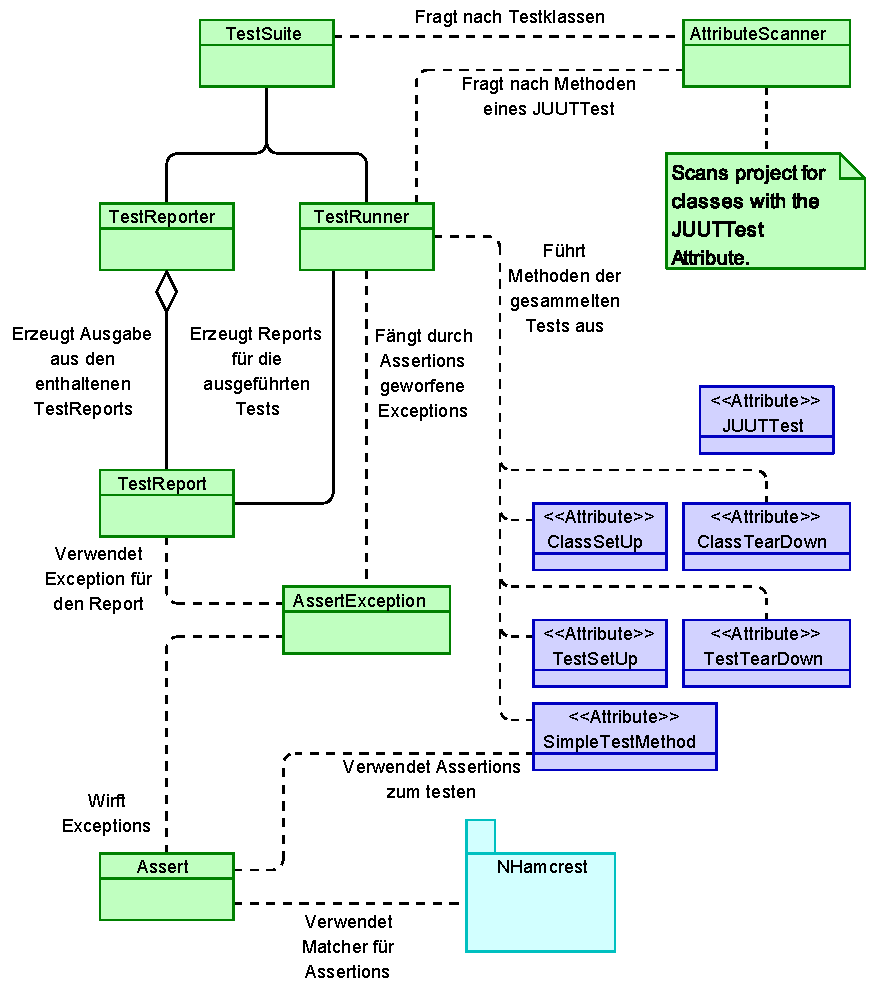
\includegraphics[width=0.9\linewidth]{images/Kapitel_ErstentwurfDesFrameworks/WalkingSkeleton}
\caption[Erstentwurf von JUUT]{Erstentwurf von JUUT}
\label{fig:WalkingSkeleton}
\end{figure}
\clearpage

Um den Aufwand für eine eigene \textit{Assert}-Klasse möglichst gering zu halten, werde ich die oben erwähnte Bibliothek NHamcrest in mein Projekt einbinden. Dabei bin ich hauptsächlich an den \textit{Matchern} interessiert, mit denen man Bedingungen, wie zum Beispiel (Un)Gleichheit zweier Objekte oder eine erwartete Exception, für die Tests definieren kann. Im Zusammenhang damit steht die \textit{AssertException}, die von \textit{Assert} geworfen wird, wenn eine solche Bedingung nicht erfüllt ist. Diese spezielle Exception soll einen fehlgeschlagenen Test markieren. Wird während des Tests eine andere Exception geworfen wird das als schwerer Fehler interpretiert.

Die Attribute dienen dazu für das Framework relevante Klassen und Methoden zu markieren, wobei ich mich an MSTest orientiert habe. Auch für JUUT sind Attribute für \textit{Class/TestSetUp}, {Class/TestTearDown}, Testmethoden und Testklassen. Das Attribut zur Markierung von Tests heißt hier \textit{SimpleTestMethod}, da für die konkreten Implementierung weitere Test-Attribute geplant sind, welche komplexer sind. Das simple Attribut ist vergleichbar mit den Tests die in UUnit oder SharpUnit möglich sind.
Neben \textit{Assert} als statische Hilfsklasse gibt es noch den \textit{AttributeScanner}. Dieser soll zum einen dazu dienen bestimmte Methoden einer Testklasse zu finden und zurückzugeben und zum anderen wäre es vorstellbar, dass er die aktuelle Umgebung nach Testklassen durchsucht. Damit ließen sich recht einfach alle Tests des aktuellen Projekts ausführen.

Der funktionale Teil besteht aus den Klassen \textit{TestSuite}, \textit{TestRunner}, \textit{TestReporter} und \textit{TestReport}. Der \textit{TestRunner} soll eine bestimmte Testklasse verwalten, an deren Methoden er mit Hilfe des \textit{AttributeScanner}s gelangt. Wird während der Ausführung eine Exception geworfen, soll diese gefangen werden und ein entsprechender \textit{TestReport} wird erzeugt. Die \textit{TestSuite} ist Zugang für den Anwender, denn hier sollen die auszuführenden Tests hinzugefügt werden. Daraufhin werden die einzelnen \textit{TestRunner} ausgeführt und deren Reports an den \textit{TestReporter} übergeben. Abschließend wird von diesem aus den gesammelten Reports eine entsprechende Ausgabe erzeugt und angezeigt.

Dieses Konzept beseitigt die oben genannten Probleme der Implementierung von UUnit, denn die Verantwortlichkeiten sind sauber verteilt und die Komplexität wird mit Hilfe der Klasse \textit{TestSuite} vor dem Anwender verborgen.